        \newpage
        
        \section*{Capítulo 4. Fundamentación del enfoque de aprendizaje profundo}
        \addcontentsline{toc}{section}{Capítulo 4. Fundamentación del enfoque de aprendizaje profundo}
        \setcounter{section}{4}
        \setcounter{subsection}{0}
        
        En este capítulo se analiza la transición del aprendizaje automático tradicional hacia el aprendizaje profundo, con el propósito de fundamentar la elección del enfoque de modelado más adecuado para el problema planteado. Para ello, se revisan los modelos básicos de clasificación, la necesidad de extracción manual de características, las limitaciones de los enfoques tradicionales y las ventajas del aprendizaje profundo en tareas visuales.
        
        \subsection{Modelos básicos de aprendizaje automático en clasificación}
        
        \subsubsection{Aprendizaje automático supervisado y clasificación}
        
        El aprendizaje automático constituye una rama de la inteligencia artificial orientada al desarrollo de modelos capaces de identificar patrones en los datos y realizar predicciones o decisiones sin haber sido programados de manera explícita para cada caso \cite{bergmann2026machine_learning}. 
        
        Dentro de este campo existen diversas técnicas que permiten abordar problemas de distinta naturaleza. En términos generales, los \textbf{métodos de machine learning} pueden clasificarse en tres paradigmas principales: \textit{aprendizaje supervisado, aprendizaje no supervisado y aprendizaje por refuerzo}. Esta división depende del objetivo con el que se entrena el modelo y, en buena medida, del tipo de datos que intervienen durante dicho proceso \cite{bergmann2026machine_learning}.
        
        Dentro de estos tres paradigmas mencionados, el que resulta de mayor interés para el presente proyecto es el \textbf{aprendizaje supervisado}, ya que el problema planteado parte de imágenes previamente etiquetadas y busca asignarles una categoría específica. Al respecto, Belcic y Stryker señalan que “el aprendizaje supervisado es una técnica de machine learning que utiliza conjuntos de datos etiquetados para entrenar modelos de inteligencia artificial (IA) para identificar los patrones y relaciones subyacentes” \cite{belcic2026supervised_learning}, de modo que el modelo aprende una relación entre un conjunto de entradas y sus salidas correspondientes, con el propósito de generalizar dicho conocimiento a nuevas muestras no vistas durante el entrenamiento.
        
        Dentro del aprendizaje supervisado las tareas se pueden dividir en  \textbf{dos tipos principales de problemas}: \textit{regresión y clasificación}. La regresión se emplea cuando la salida esperada corresponde a la predicción de un valor continuo, con base en el análisis de las relación entre variables dependientes e independientes, mientras que la clasificación se utiliza cuando el objetivo consiste en asignar una nueva muestra a una categoría previamente definida o también llamada clase \cite{belcic2026supervised_learning}. En este sentido, el problema abordado en el presente trabajo corresponde a una tarea de clasificación (tal como se definió en el capítulo anterior), con enfoque supervisado, ya que se busca determinar si una imagen de un árbol presenta o no indicios visuales de infestación por plaga.
        
        \subsubsection{Principales algoritmos de clasificación}
        
        Una vez establecido que el problema abordado en este trabajo corresponde a una tarea de clasificación, resulta pertinente revisar los tipos de clasificación y algunos de los algoritmos que tradicionalmente se han utilizado para resolver este tipo de problemas dentro del aprendizaje automático supervisado. 
        
        Este tipo de tarea puede presentarse de distintas maneras. Por un lado, se encuentra la \textbf{clasificación binaria}, en la que el modelo debe decidir entre dos clases posibles; por otro, la \textbf{clasificación multiclase}, donde la tarea consiste en elegir una categoría entre varias opciones. En problemas más específicos también puede hablarse de clasificación multietiqueta, aunque esta variante no corresponde al alcance del presente trabajo \cite{belcic2026classification_ml}.

        Dentro de los algoritmos de clasificación más conocidos se encuentra la \textbf{regresión logística}, la cual se emplea con frecuencia en problemas de clasificación binaria debido a su capacidad para estimar la probabilidad de pertenencia a una clase. También destacan los \textbf{árboles de decisión}, que estructuran la toma de decisiones mediante reglas jerárquicas construidas a partir de las características de entrada. A partir de estos, surgen métodos como el \textbf{bosque aleatorio}, que combina múltiples árboles para mejorar la capacidad de generalización del modelo y reducir la dependencia de un solo esquema de decisión \cite{belcic2026classification_ml}.
        
        Otro algoritmo ampliamente utilizado es la \textbf{máquina de vectores de soporte} (Support Vector Machine, SVM), cuyo propósito es encontrar una frontera de separación adecuada entre clases dentro del espacio de características. De manera similar, el método de \textbf{k-vecinos más cercanos}(k-Nearest Neighbors, k-NN) clasifica una observación de acuerdo con la cercanía que guarda respecto a muestras previamente etiquetadas. Asimismo, el clasificador de \textbf{Bayes ingenuo}(Naive Bayes) constituye un enfoque probabilístico que asigna clases con base en la probabilidad de ocurrencia de ciertas características dentro de cada categoría \cite{belcic2026classification_ml}.

\begin{figure}[H]
    \centering
    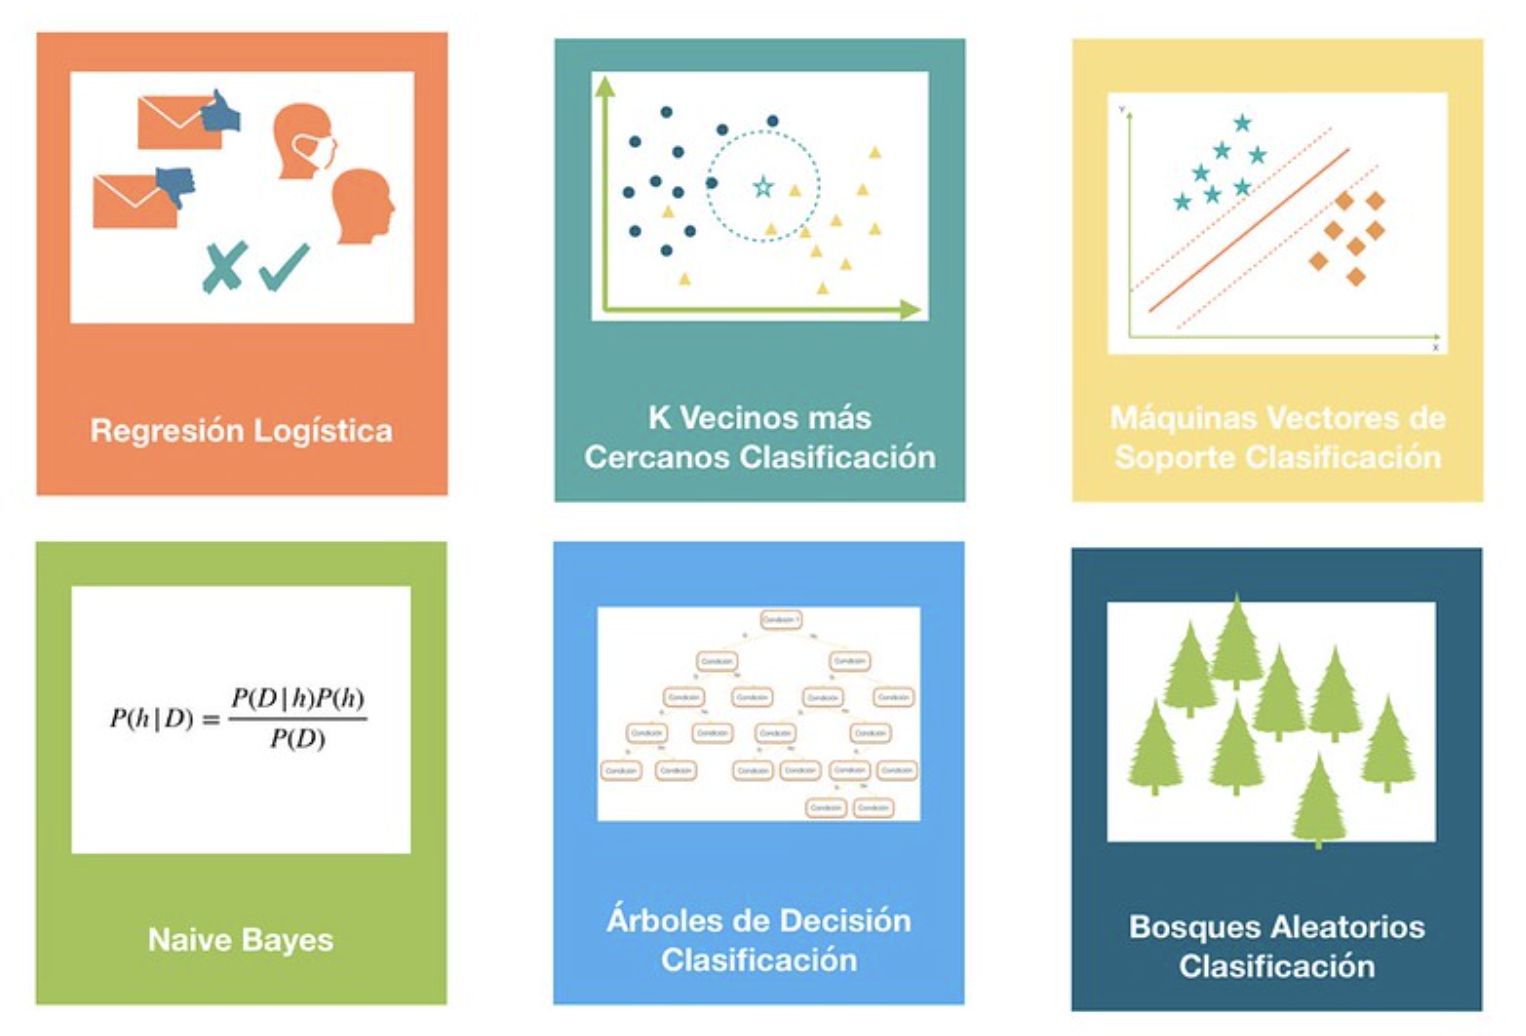
\includegraphics[width=0.8\textwidth]{images/C4/algClasi.png}
    \caption{Principales algoritmos de clasificación. Tomado de \cite{aprendeia2019ventajas_desventajas_clasificacion}}
    
\end{figure}
